\chapter{Esperimenti e Risultati}
\label{chap_exp}
In questo capitolo verranno descritti gli esperimenti e i risultati del lavoro. In particolare, verranno descritti alcuni dettagli implementativi, come le librerie e i framework utilizzati, ma anche le risorse computazionali sfruttate. Inoltre, verranno descritte nel dettaglio le strategie adottate durante l'addestramento, gli iperparametri e i vari metodi testati negli esperimenti.

%\section{Regolarizzazione}
%Come descritto nel paragrafo \ref{regolarizzazione}, uno degli aspetti più importanti e difficili dell'addestare una rete neurale è quello della regolarizzazione. In particolare, per far fronte al problema dell'overfitting e viste le difficoltà che il dataset FloodNet presenta, durante il lavoro sono stati utilizzati diversi metodi di regolarizzazione. In particolare, le principali tecniche di regolarizzazione utilizzate sono il dropout \ref{regolarizzazione} e la data augmentation \ref{data_augmentation}.




\section{Risorse computazionali}
\label{risorse_comp}
Dato che l'addestramento di una rete neurale comporta un costo computazionale molto elevato, non avendo disponibilità di una macchina locale con abbastanza potenza computazionale per riuscire ad addestrare il modello in tempi accettabili, è stata utilizzata una nota piattaforma, chiamata Google Colab. In particolare, Google Colab permette di eseguire codice da remoto su delle macchine virtuali equipaggiate con potenza di calcolo elevata, dando soprattutto accesso a macchine virtuali con GPU, che sono fondamentali per l'addestramento di una rete neurale. Purtroppo però, Google Colab presenta delle forti limitazioni, non tanto dal punto di vista di potenza computazionale delle risorse, bensì dal punto di vista della loro disponibilità. Nello specifico, per poter offrire gratuitamente risorse computazionali e accogliere l'elevato numero di richieste, la disponibilità di risorse hardware subisce forti fluttuazioni.
In particolare, teoricamente la vita massima di una macchina virtuale utlizzata è di 12 ore. Nella pratica però questo numero è sempre inferiore, sia per le fluttuazioni di richieste menzionate precedentemente, sia a causa di altri meccanismi:

\begin{itemize}
    \item I notebook utilizzati per eseguire il codice hanno un timeout di inattività. Di conseguenza, soprattutto per l'addestramento di una rete neurale, che comporta dei lunghi tempi passivi, questo aspetto è risultato fortemente limitante.
    
    \item L'utilizzo delle GPU vengono priorizzate per gli utenti che utilizzano Colab in modo più interattivo. Anche qui, troviamo un forte contrasto con la tipologia di utilizzo che riguarda l'addestramento di una rete neurale.
\end{itemize}

Di conseguenza, visti tutti questi aspetti, le risorse di Google Colab non sono state né garantite né sempre disponibili. Questo vuol dire che, durante il lavoro la disponibilità delle risorse necessarie a portare avanti gli esperimenti, ha avuto notevoli limitazioni, causando di conseguenza grandi rallentamenti. Nella pratica, le risorse hardware di Google Colab sono state disponibili per una media di circa 5/6 ore giornaliere.
Le specifiche tecniche dell'hardware fornito sono le seguenti:

\begin{itemize}
    \item  \textbf{CPU}: Intel(R) Xeon(R)
    \item \textbf{RAM}: 12GB
    \item \textbf{GPU}: NVIDIA K80 12 GB
\end{itemize}





\section{Tecnologie usate}
Per quanto riguarda l'implementazione di tutte le metodologie, sono state utilizzate svariate librerie e framework. 
In particolare, le principali utilizzate sono:

\begin{itemize}
    \item \textbf{PyTorch}: un framework open source di Machine Learning basato sul linguaggio di programmazione Python e sulla libreria Torch. È uno dei framework più utilizzati nel campo del Deep Learning, insieme a Tensorflow.
    
    \item \textbf{CUDA (Compute Unified Device Architecture)}: un’architettura hardware per il calcolo parallelo sviluppata da NVIDIA. In particolare, CUDA permette di sfruttare al meglio la potenza di calcolo di una GPU, parallelizzando le computazioni in modo efficiente e il risultato è che le prestazioni, soprattutto per quanto riguarda la fase di addestramento e di inferenza, sono superiori a quelle di una CPU.
    
    \item \textbf{Albumentations} \cite{albumentations}: un tool di Computer Vision basato sul linguaggio di programmazione Python, che ha lo scopo di rendere la data augmentation veloce e flessibile. Esso implementa in modo efficiente una ricca varietà di trasformazioni dell'immagine, ottimizzate per le prestazioni, fornendo un'interfaccia di data augmentation concisa ma potente per diversi task di Computer Vision, tra cui la classificazione, segmentazione, object detection e altri.
    
    \item \textbf{OpenCV (Open Source Computer Vision Library}): una libreria open source di Computer Vision e Machine Learning costruita per fornire un'infrastruttura comune per le applicazioni di Computer Vision e per accelerare l'uso della \textit{machine perception} nei prodotti commerciali.
\end{itemize}


\section{Dataset FloodNet}
Per l'addestramento e la valutazione dei metodi e delle architetture usate in questo lavoro, è stato utilizzato il dataset \textit{FloodNet} \cite{floodnet}. In particolare, questo dataset è stato pubblicato nel 2021 a seguito della FloodNet Challenge del workshop EARTHVISION 2021 tenuto dal CVPR 2021 (Computer Vision and Pattern Recognition Conference), uno dei principali eventi annuali di Computer Vision, che comprende numerose conferenze e workshops. Floodnet è stato uno dei primi dataset pubblici del suo genere: in particolare, è stato il primo dataset pubblico con immagini e video di UAV ad alta risoluzione e a bassa altitudine, riguardanti la fase immediatamente successiva ad un disastro naturale. Inoltre, FloodNet è uno dei pochi dataset in questo ambito a poter essere utilizzato per ben tre task differenti, ovvero classificazione, segmentazione semantica e VQA (Visual Question Answering).
Le immagini del dataset sono state catturate tra il 30 Agosto e il 4 Settembre del 2017 in Texas (USA), immediatamente dopo il disastro causato dall'Uragano Harvey, con un quadricottero DJI Mavic Pro a 200 piedi di altitudine. In totale sono state raccolte 2343 immagini con una risoluzione di 1.5cm per pixel. Per quanto riguarda il task della segmentazione, ogni  pixel di ogni immagine è stata annotata con una delle 9 classi ("edificio allagato", "edificio non allagato", "strada allagata", "strada non allagata", "acqua", "albero", "veicolo", "piscina" e "prato").
Come detto in precedenza, FloodNet, al momento della sua pubblicazione, è risultato un dataset unico nel suo genere. In particolare, prima della sua pubblicazione la maggior parte dei dataset pubblici con immagini riguardanti disastri naturali erano di origine satellitare. Il problema di questo tipo di immagini è che spesso, per ottenere questo tipo di dato, le attese sono di diversi giorni e dunque non si hanno dati fedeli alla fase immediatamente successiva al disatro. Inoltre, la loro risoluzione è chiaramente molto più bassa rispetto alle immagini a bassa altitudine, di conseguenza spesso scarseggiano di informazioni dettagliate sui danni causati dall'evento. Il dataset viene fornito già diviso nelle tre parti di training, validation e testing, con le seguenti proporzioni: $\sim60\%$ per il training set, $\sim20\%$ per il validation set e $\sim20\%$ per il test set. 
Come già menzionato nel paragrafo \ref{data_aug_used}, durante il lavoro il numero delle immagini totali che compongono il dataset ha subito delle variazioni. In particolare, il dataset ha avuto tre versioni: una versione all'interno della quale sono state scartate tutte le 182 immagini trovate con errori importanti, per un totale di 2161 immagini; una versione dove di queste 182, 137 sono state corrette e reinserite, per un totale 2298; e infine un'ultima versione dove oltre a quelle corrette, sono state aggiunte 420 immagini, frutto della data augmentation offline, per un totale di 2718 immagini. Nella Figura \ref{fig:example_ds} vengono mostrati alcuni esempi delle immagini e maschere presenti nel dataset FloodNet.

\begin{figure}
    \hspace*{-0.3cm}
    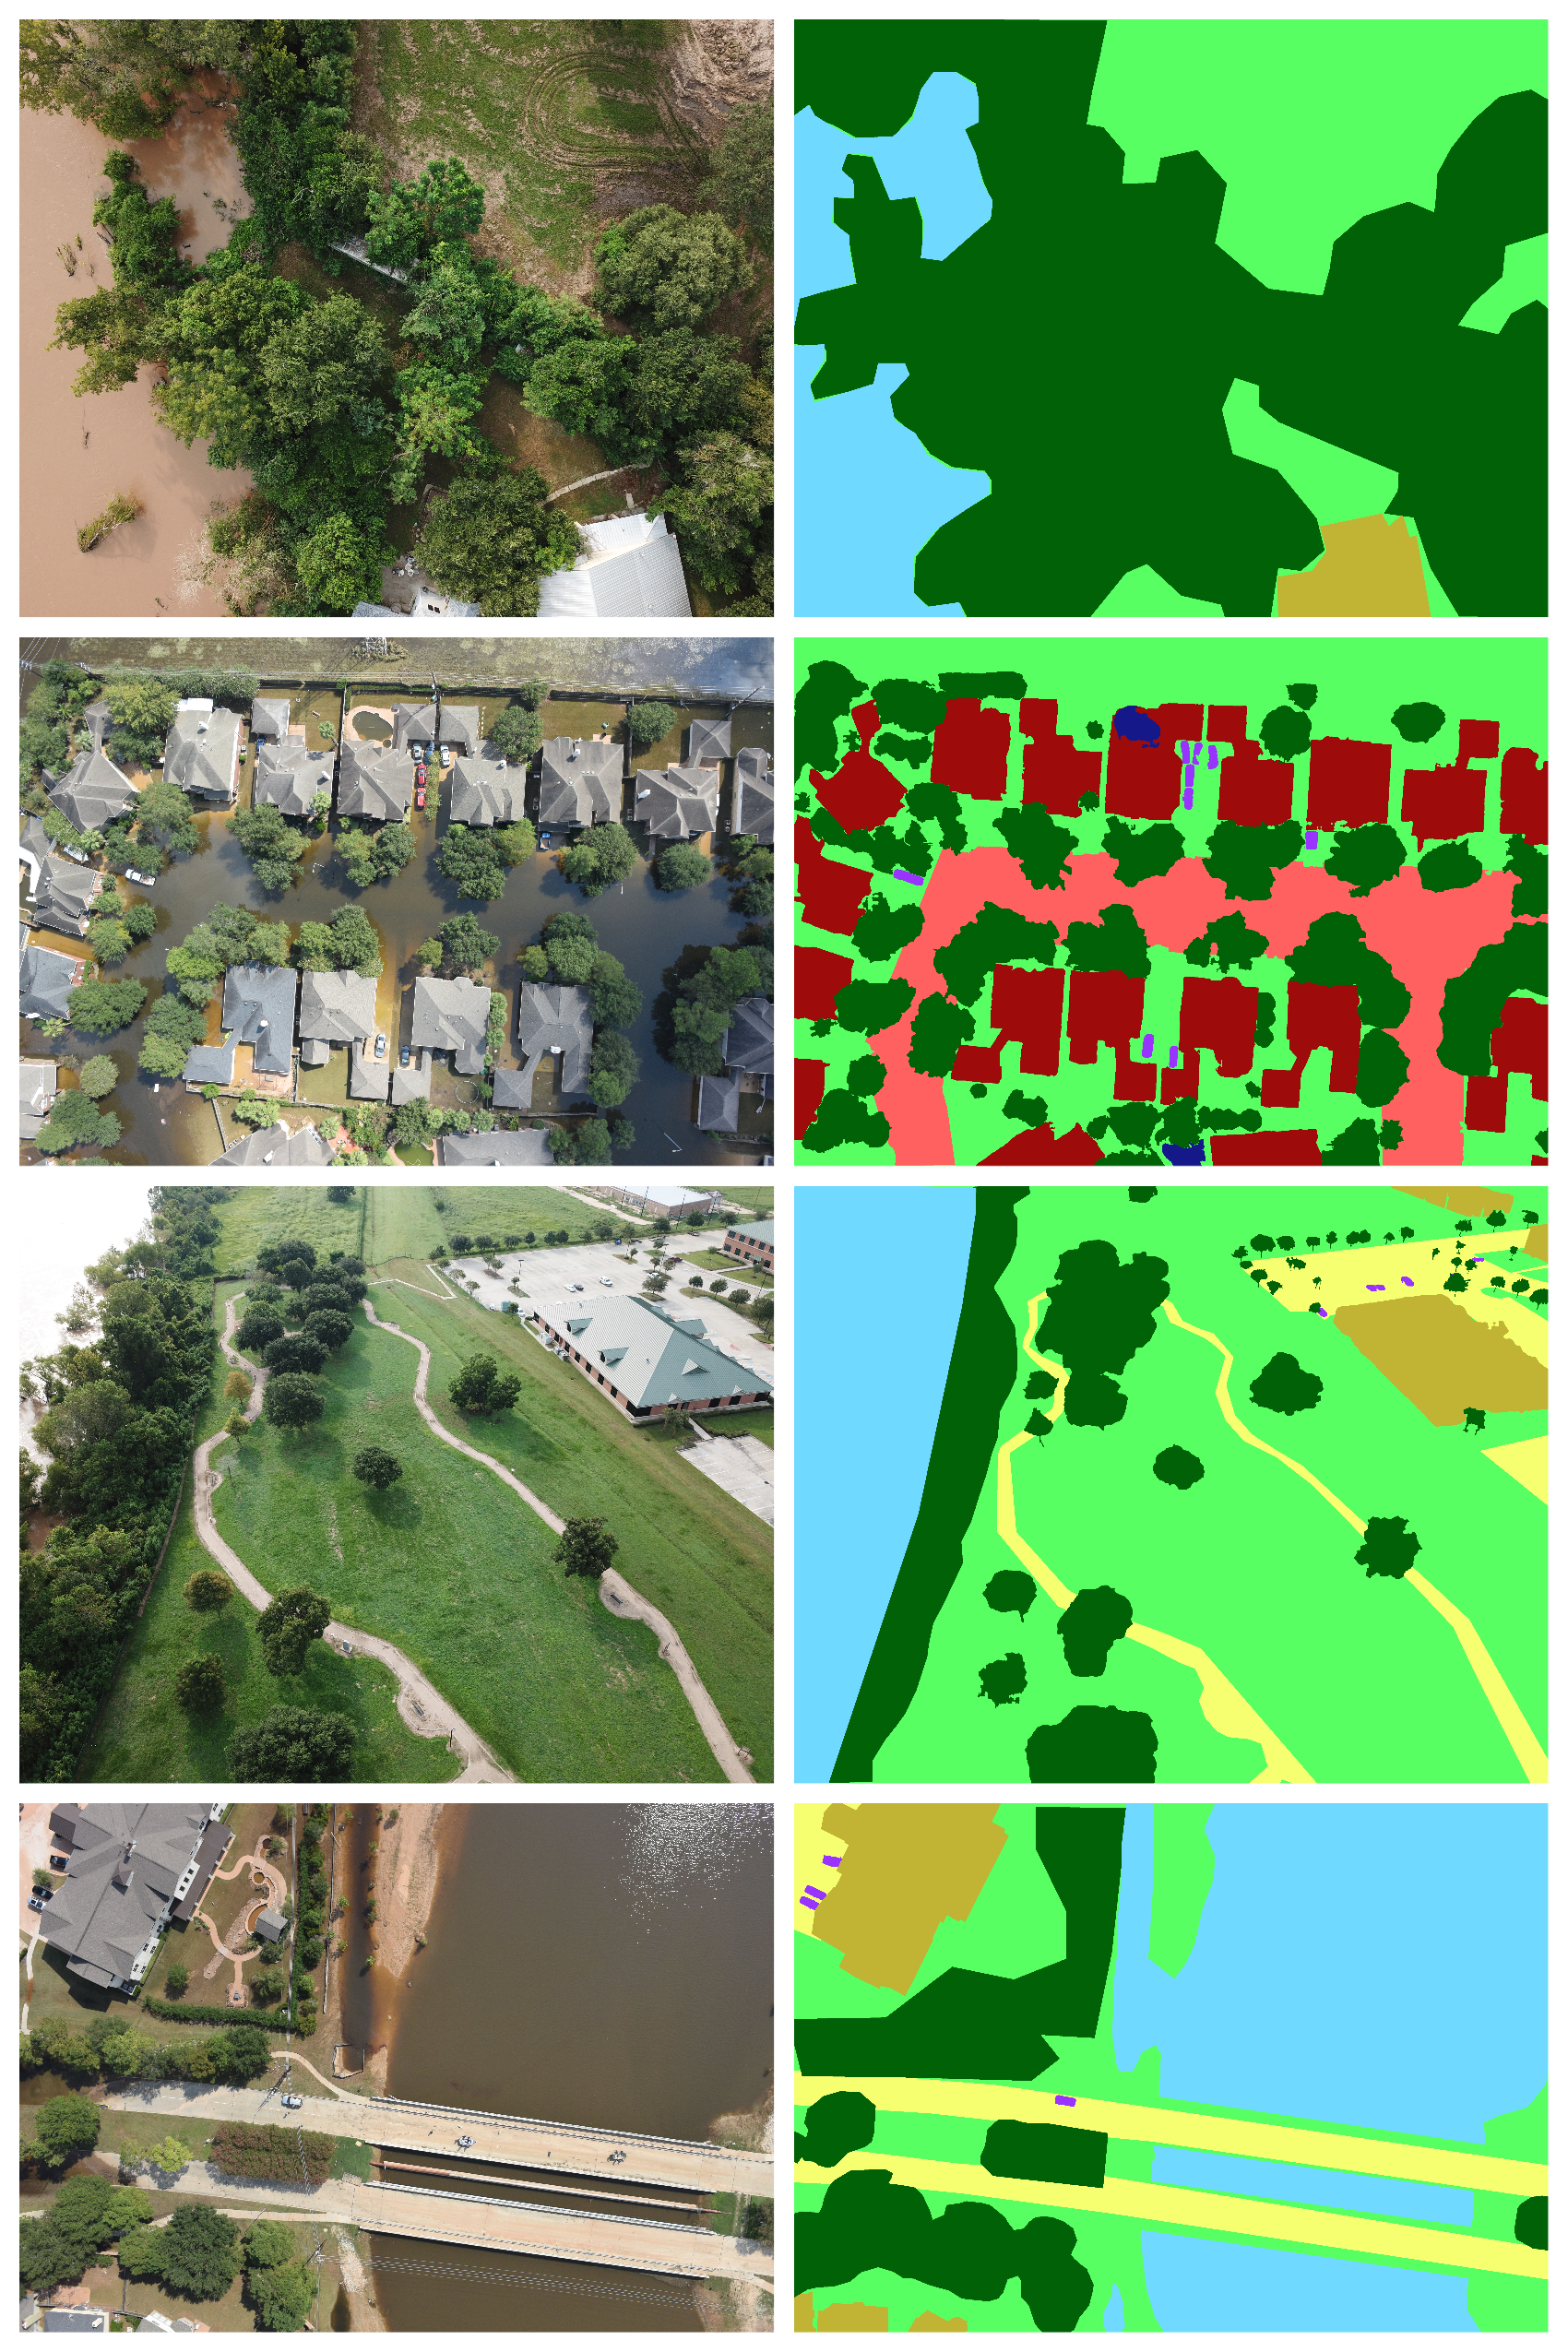
\includegraphics[scale=0.25]{img/esempi_img_ds.jpg}
    \caption{Alcuni esempi delle immagini (a sinistra) del dataset FloodNet con abbinate le corrispondenti maschere (a destra).}
    \label{fig:example_ds}
\end{figure}


    
%\section{Dataset FloodNet}

    
    
    


\section{Esperimenti}
I principali esperimenti effettuati sono quattro. Nel primo è stato testato il modello DeepLabV3 sulla prima versione del dataset, ovvero quella da 2161 immagini totali. Nello specifico, al di là della regolarizzazione fatta con il dropout, non è stata utilizzata nessuna particolare strategia o tecnica. L'obiettivo infatti, era quello di impostare una baseline da cui poi cercare di migliorare. Le immagini sono state ridimensionate a 600*800, è stata usata una \textit{batch size} di 2, un learning rate di 0.01, l'ottimizzatore Adam e la funzione di perdita Focal Loss. La tabella \ref{table:config1_mIoU} mostra i risultati e come si può notare, sulla maggior parte delle classi il modello ottiene performance scarse. La motivazione, probabilmente, risiede nel fatto che utilizzando questa versione del dataset, molte classi risultano troppo poco presenti nelle immagini e inoltre, senza nessun tipo particolare di regolarizzazione (tranne il dropout), il modello fatica a generalizzare.


\begin{table}[h!]
%\centering
\hspace{-0.1in}
\begin{tabular}{||p{1cm} p{1cm} p{1cm} p{1cm} p{1cm} p{1cm} p{1cm} p{1cm} p{1cm} | p{1cm}||}
 \hline
    Classe 1 & Classe 2 & Classe 3 & Classe 4 & Classe 5 & Classe 6 & Classe 7 & Classe 8 & Classe 9 & mIoU \\ [0.5ex]
 \hline
0.0018 & 0.087 & 0.0002 & 0.28 &  0.14 & 0.339 & 0.006 & 0.0 & 0.309 & 0.129 \\ [1ex] 
 \hline
\end{tabular}
\caption{Risultati del primo esperimento. La tabella \ref{table:class_legend} mostra la legenda delle classi.}
\label{table:config1_mIoU}
\end{table}


\begin{table}[h!]
\centering
%\hspace{-0.77in}
\begin{tabular}{||c | c||}
 \hline
    Classe 1 & Edificio allagato \\ [0.5ex]
    Classe 2 & Edificio non allagato \\ [0.5ex]
    Classe 3 & Strada allagata \\ [0.5ex]
    Classe 4 & Strada non allagata \\ [0.5ex]
    Classe 5 & Acqua \\ [0.5ex]
    Classe 6 & Albero \\ [0.5ex]
    Classe 7 & Veicolo \\ [0.5ex]
    Classe 8 & Piscina \\ [0.5ex]
    Classe 9 & Prato \\ [0.5ex]
 \hline
\end{tabular}
\caption{Legenda delle classi.}
\label{table:class_legend}
\end{table}

Nel secondo esperimento è stata introdotta la fase di data augmentation online di cui si è parlato nel paragrafo \ref{data_aug_used}. Inoltre, è stato applicato anche un metodo di normalizzazione dell'input, ovvero tutti e tre i canali dell'RGB sono stati divisi per 255. Lo scopo di questa normalizzazione è di portare l'input dal range $[0, 255]$ a $[0, 1]$,  e così facendo si velocizza l'addestramento, ottenendo di conseguenza un modello migliore con lo stesso numero di epoche. Il funzionamento di questo meccanismo si basa sul fatto che normalizzando l'input, la funzione di costo che cerchiamo di minimizzare durante l'addestramento prende una forma che si rivela più semplice da ottimizzare. Oltre a questo, gli iperparametri del primo esperimento rimangono invariati. La tabella \ref{table:config5_mIoU} mostra i risultati di questa configurazione. Come si può notare, la normalizzazione e soprattutto l'aggiunta della data augmentation online hanno portato un leggero miglioramento, ma le performance risultano ancora scarse, soprattutto sulle classi più difficoltose, ovvero "edificio allagato", "strada allagata", "veicolo" e "piscina".

\begin{table}[h!]
%\centering
\hspace{-0.1in}
\begin{tabular}{||p{1cm} p{1cm} p{1cm} p{1cm} p{1cm} p{1cm} p{1cm} p{1cm} p{1cm} | p{1cm}||}
 \hline
    Classe 1 & Classe 2 & Classe 3 & Classe 4 & Classe 5 & Classe 6 & Classe 7 & Classe 8 & Classe 9 & mIoU \\ [0.5ex]
 \hline
0.0003 & 0.12 & 0.001 & 0.27 &  0.23 & 0.38 & 0.0 & 0.03 & 0.52 & 0.175 \\ [1ex] 
 \hline
\end{tabular}
\caption{Risultati del secondo esperimento.}
\label{table:config5_mIoU}
\end{table}

Nel terzo esperimento invece, viene utilizzata la seconda versione del dataset, ovvero quella da 2298 immagini, all'interno della quale sono state reinserite le maschere corrette. Oltre a questo, si è cercato di alzare il più possibile la risoluzione delle immagini, in quanto, alcune classi come "veicolo", essendo rappresentate da oggetti molto piccoli, risultano fortemente svantaggiate dal ridimensionamento delle immagini. In particolare, essendo limitati dalle risorse computazionali e cercando di mantenere una batch size di minimo 2, la risoluzione è stata alzata a 750*1000. La tabella \ref{table:config8_mIoU} mostra i risultati di questo terzo esperimento. Come si può notare, l'applicazione di queste due strategie ha portato un netto miglioramento, sia per quanto riguarda le classi più semplici, ma soprattutto per quanto riguarda quelle più difficoltose. La motivazione, oltre al fatto che alzando la risoluzione il modello riceve più informazioni, è soprattutto che, grazie alla pulizia e correzione del dataset si è reintrodotto un numero importante di immagini. Nello specifico, non è tanto il numero totale di immagini aggiunte ad aver fatto la differenza, ma piuttosto il fatto che la maggior parte di queste immagini contenevano soprattutto le classi su cui si avevano le performance più scarse. Infatti, come viene mostrato nella Tabella \ref{table:config8_vs_config5}, le classi che hanno avuto in proporzione un miglioramento più grande, sono "edificio allagato", "strada allagata", "veicolo" e "piscina". Anche qui, gli iperparametri come learning rate, batch size, ottimizzatore e funzione di perdita sono rimasti invariati.

\begin{table}[h!]
%\centering
\hspace{-0.1in}
\begin{tabular}{||p{1cm} p{1cm} p{1cm} p{1cm} p{1cm} p{1cm} p{1cm} p{1cm} p{1cm} | p{1cm}||}
 \hline
    Classe 1 & Classe 2 & Classe 3 & Classe 4 & Classe 5 & Classe 6 & Classe 7 & Classe 8 & Classe 9 & mIoU \\ [0.5ex]
 \hline
0.14 & 0.47 & 0.06 & 0.48 &  0.46 & 0.55 & 0.34 & 0.26 & 0.81 & 0.402 \\ [1ex] 
 \hline
\end{tabular}
\caption{Risultati del terzo esperimento esperimento.}
\label{table:config8_mIoU}
\end{table}

\begin{table}[h!]
%\centering
\hspace{-0.3in}
\begin{tabular}{||p{1.5cm} p{1cm} p{1.5cm} p{1cm} p{1cm} p{1cm} p{1cm} p{1cm} p{1cm} | p{1.2cm}||}
 \hline
    Classe 1 & Classe 2 & Classe 3 & Classe 4 & Classe 5 & Classe 6 & Classe 7 & Classe 8 & Classe 9 & mIoU \\ [0.5ex]
 \hline
+46500\% & +291\% & +5900\% & +77\% & +100\% & +44\% & (inf) & +766\% & +55\% & +129\% \\ [1ex] 
 \hline
\end{tabular}
\caption{Miglioramenti avuti nel terzo esperimento rispetto al secondo.}
\label{table:config8_vs_config5}
\end{table}




Infine, nel quarto ed ultimo esperimento, viene utilizzata l'ultima versione del dataset, ovvero quello da 2718 immagini totali, frutto della data augmentation offline.
La tabella \ref{table:config9_mIoU_1} mostra i risultati. Anche qui troviamo un netto miglioramento rispetto alla configurazione precedente su tutte le classi, ma soprattutto, come viene mostrato nella Tabella \ref{table:config8_vs_config9}, sulle due classi "edificio allagato" e "strada allagata".
Anche qui la motivazione principale è che, grazie all'aggiunta di immagini contenenti soprattutto queste due classi, il modello ha più materiale per apprenderle.

\begin{table}[h!]
%\centering
\hspace{-0.1in}
\begin{tabular}{||p{1cm} p{1cm} p{1cm} p{1cm} p{1cm} p{1cm} p{1cm} p{1cm} p{1cm} | p{1cm}||}
 \hline
    Classe 1 & Classe 2 & Classe 3 & Classe 4 & Classe 5 & Classe 6 & Classe 7 & Classe 8 & Classe 9 & mIoU \\ [0.5ex]
 \hline
0.32 & 0.51 & 0.24 & 0.55 &  0.55 & 0.6 & 0.4 & 0.44 & 0.84 & 0.5 \\ [1ex] 
 \hline
\end{tabular}
\caption{Risultati del quarto esperimento esperimento.}
\label{table:config9_mIoU_1}
\end{table}

\begin{table}[h!]
%\centering
\hspace{-0.3in}
\begin{tabular}{||p{1.5cm} p{1cm} p{1.5cm} p{1cm} p{1cm} p{1cm} p{1cm} p{1cm} p{1cm} | p{1.2cm}||}
 \hline
    Classe 1 & Classe 2 & Classe 3 & Classe 4 & Classe 5 & Classe 6 & Classe 7 & Classe 8 & Classe 9 & mIoU \\ [0.5ex]
 \hline
+128\% & +8\% & +300\% & +14\% & +19\% & +9\% & +17 & +69\% & +3\% & +24\% \\ [1ex] 
 \hline
\end{tabular}
\caption{Miglioramenti avuti nel quarto esperimento rispetto al terzo.}
\label{table:config8_vs_config9}
\end{table}

Visti i miglioramenti apportati con questa configurazione, si è deciso di spingere il più possibile la fase di addestramento. In particolare, ispirandosi al lavoro di \cite{deeplabv1, deeplabv2, deeplabv3} si è adottata la seguente strategia: a partire dalla settecentesima epoca, si è fatto diminuire il learning rate ogni 100 epoche, moltiplicandolo per 0.1. Spingendo l'addestramento fino a 1000 epoche si sono ottenuti i risultati mostrati nella Tabella \ref{table:config9_mIoU_2}. Nello specifico, quest'ultimo addestramento ha richiesto un tempo totale di circa 350 ore, che a causa delle limitazioni dal punto di vista delle risorse computazionali (Paragrafo \ref{risorse_comp}), sono state suddivise in circa 5/6 ore giornaliere, portando a un tempo totale di addestramento di circa 60 giorni.


\begin{table}[h!]
%\centering
\hspace{-0.1in}
\begin{tabular}{||p{1cm} p{1cm} p{1cm} p{1cm} p{1cm} p{1cm} p{1cm} p{1cm} p{1cm} | p{1cm}||}
 \hline
    Classe 1 & Classe 2 & Classe 3 & Classe 4 & Classe 5 & Classe 6 & Classe 7 & Classe 8 & Classe 9 & mIoU \\ [0.5ex]
 \hline
0.41 & 0.60 & 0.32 & 0.6 &  0.57 & 0.65 & 0.49 & 0.52 & 0.86 & 0.564 \\ [1ex] 
 \hline
\end{tabular}
\caption{Risultati del quinto esperimento.}
\label{table:config9_mIoU_2}
\end{table}


Infine, la Figura \ref{fig:ground_vs_inference} mostra un esempio di paragone tra le maschere corrette e l'output del modello.


\begin{figure}[h!]
     \centering
     \begin{subfigure}[b]{0.45\textwidth}
         \centering
         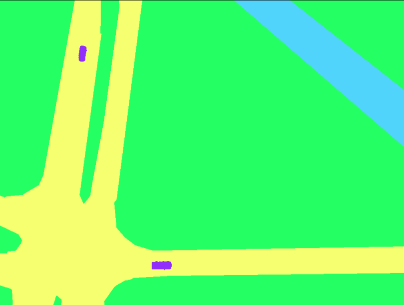
\includegraphics[width=\textwidth]{img/1_1.png}
         \caption{}
         \label{}
     \end{subfigure}
     \hfill
     \begin{subfigure}[b]{0.45\textwidth}
         \centering
         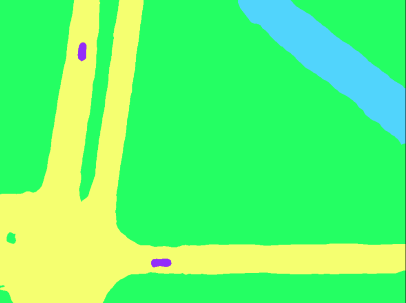
\includegraphics[width=\textwidth]{img/1_2.png}
         \caption{}
         \label{}
     \end{subfigure}
     \hfill
     \begin{subfigure}[b]{0.45\textwidth}
         \centering
         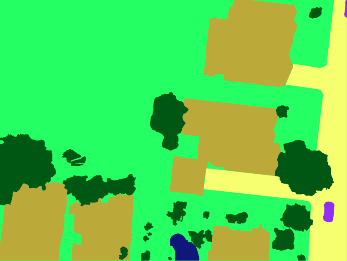
\includegraphics[width=\textwidth]{img/2_1.png}
         \caption{}
         \label{}
     \end{subfigure}
     \hfill
     \begin{subfigure}[b]{0.45\textwidth}
         \centering
         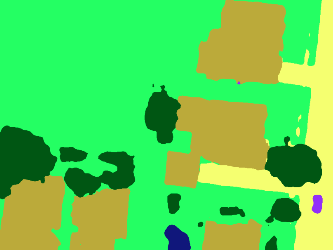
\includegraphics[width=\textwidth]{img/2_2.png}
         \caption{}
         \label{}
     \end{subfigure}
     \hfill
     \begin{subfigure}[b]{0.45\textwidth}
         \centering
         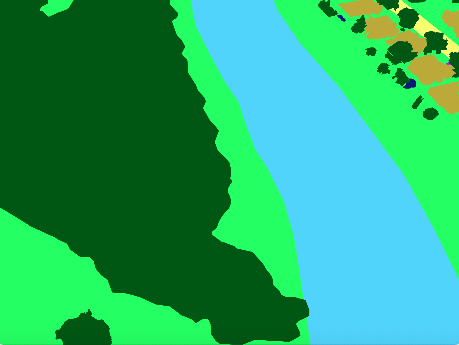
\includegraphics[width=\textwidth]{img/3_1.png}
         \caption{}
         \label{}
     \end{subfigure}
     \hfill
     \begin{subfigure}[b]{0.45\textwidth}
         \centering
         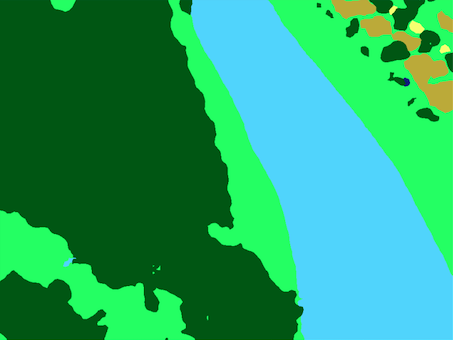
\includegraphics[width=\textwidth]{img/3_2.png}
         \caption{}
         \label{fig:three sin x}
     \end{subfigure}
     \hfill
     \begin{subfigure}[b]{0.45\textwidth}
         \centering
         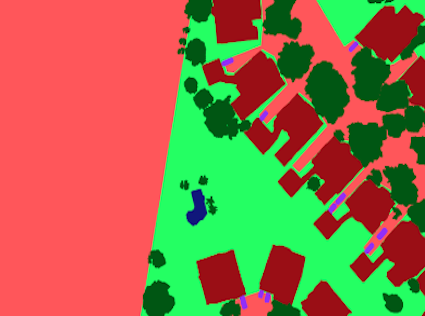
\includegraphics[width=\textwidth]{img/4_1.png}
         \caption{}
         \label{}
     \end{subfigure}
     \hfill
     \begin{subfigure}[b]{0.45\textwidth}
         \centering
         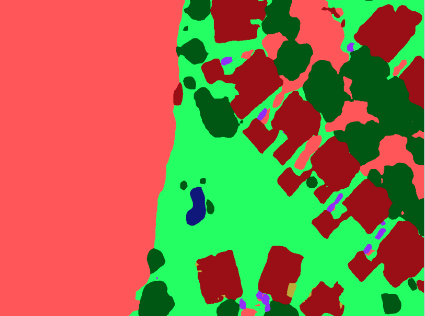
\includegraphics[width=\textwidth]{img/4_2.png}
         \caption{}
         \label{}
     \end{subfigure}
        \caption{Le otto immagini mostrano un esempio di paragone tra le maschere corrette (a), (c), (e), (g) e le maschere prodotte dal modello (b), (d), (f), (h).}
        \label{fig:ground_vs_inference}
\end{figure}















\section{Paragone con altri lavori}
\label{comparison}
Nella Tabella \ref{table:paragone} viene riportato il paragone tra il metodo proposto e un altro lavoro dello stato dell'arte \cite{floodnet} che riguarda lo stesso dataset. 
Un fattore molto importante da considerare nel paragonare i risultati di questo lavoro con quelli di \cite{floodnet}, è che la loro versione del dataset contiene 3200 immagini totali, a fronte delle 2343 della versione di questo lavoro. Dunque, la loro versione del dataset presenta un +36\% di immagini totali, il che comporta inevitabilmente un importante vantaggio nella fase di addestramento. Questo è anche comprovato dal fatto che, nel metodo proposto, sia con la fase di pulizia del dataset sia con quella di data augmentation offline, aggiungendo corrispettivamente +6\% e +18\% di immagini, si sono ottenuti importanti miglioramenti, dimostrando dunque il vantaggio di avere a disposizione il 36\% di immagini aggiuntive. Un loro ulteriore vantaggio è stato dal punto di vista delle risorse computazionali. In particolare, a differenza di questo lavoro che, come già detto, è stato fortemente rallentato per le ragioni sopra citate (Paragrafo \ref{risorse_comp}), il loro lavoro si è basato sulla disponibilità continua di una macchina locale con la GPU Nvidia GeForce RTX 2080 Ti. La disponibilità continua di potenza computazionale che una macchina locale fornisce, rappresenta un importante vantaggio, soprattutto se paragonato ad una disponibilità di 5/6 ore giornaliere. 

%Inoltre, nella Tabella \ref{table:paragone_deeplabv3+} viene evidenziato il paragone con il modello DeepLabV3+, molto simile a quello utilizzato in questo lavoro. 


Inoltre, sempre dalla Tabella \ref{table:paragone} si può notare che, nonostante lo svantaggio derivante da una minor disponibilità di immagini e da una ridotta accessibilità alle risorse computazionali, il metodo proposto migliora le IoU delle quattro classi "edificio allagato", "veicolo", "piscina" e "prato". Inoltre, un importante fattore da considerare è che le classi "edificio allagato", "veicolo" e "piscina" sono tre delle quattro, insieme a "strada allagata", che durante il lavoro si sono rivelate le più difficili da apprendere. Infine, tutti gli aspetti menzionati precedentemente dimostrano che il metodo proposto è promettente e che con risorse più adeguate e con un dataset più esteso, potrebbe raggiungere performance più alte.


%Infine, entrambi questi aspetti dimostrano che i risultati di questo lavoro si possono considerare più che soddisfacenti.



\begin{table}[h!]
%\centering
\hspace{-0.7in}
\begin{tabular}{||p{2.3cm} | p{1cm} p{1cm} p{1cm} p{1cm} p{1cm} p{1cm} p{1cm} p{1cm} p{1cm} | p{1cm}||}
 \hline
    Modello & Classe 1 & Classe 2 & Classe 3 & Classe 4 & Classe 5 & Classe 6 & Classe 7 & Classe 8 & Classe 9 & mIoU \\ [0.5ex]
 \hline\hline
 \hline
ENet & 0.069 & 0.473 & 0.124 & 0.484 &  0.489 & 0.683 & 0.322 & 0.424 & 0.762 & 0.426 \\ [1ex] 
 \hline
DeepLabV3+ & 0.327 & 0.728 & 0.52 & 0.7 &  0.75 & 0.77 & 0.42 & 0.47 & 0.84 & 0.61 \\ [1ex]
\hline
\textbf{DeepLabV3} & \textbf{0.41 }& 0.60 & 0.32 & 0.6 &  0.57 & 0.65 & \textbf{0.49} & \textbf{0.52} & \textbf{0.86} & 0.564 \\ [1ex]
% \hline
%PSPNet &  0.68 & 0.89 & 0.82 & 0.91 &  0.92 & 0.89 & 0.46 & 0.64 & 0.93 & 0.79 \\ [1ex]
 \hline
\end{tabular}
\caption{Paragone tra l'approccio sviluppato e quello di \cite{floodnet}.}
\label{table:paragone}
\end{table}




%\begin{table}[h!]
%\centering
%\hspace{-0.7in}
%\begin{tabular}{||p{2.3cm} | p{1cm} p{1cm} p{1cm} p{1cm} p{1cm} p{1cm} p{1cm} p{1cm} p{1cm} | p{1cm}||}
% \hline
%    Modello & Classe 1 & Classe 2 & Classe 3 & Classe 4 & Classe 5 & Classe 6 & Classe 7 & Classe 8 & Classe 9 & mIoU \\ [0.5ex]
% \hline\hline
 %\hline
%\textbf{DeepLabV3} & \textbf{0.41} & 0.60 & 0.32 & 0.6 &  0.57 & 0.65 & \textbf{0.49} & \textbf{0.52} & 0.86 & 0.564 \\ [1ex]  
 %\hline
%DeepLabV3+ & 0.327 & 0.728 & 0.52 & 0.7 &  0.75 & 0.77 & 0.42 & 0.47 & 0.84 & 0.61 \\ [1ex]
 %\hline
%\end{tabular}
%\caption{Paragone tra l'approccio sviluppato e un modello molto simile dello stato dell'arte (DeepLabV3+), utilizzato in \cite{floodnet}.}
%\label{table:paragone_deeplabv3+}
%\end{table}


